\begin{center}
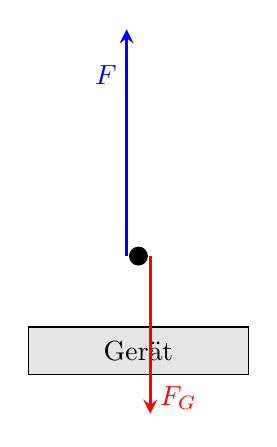
\begin{tikzpicture}[>=stealth]
 \draw[fill=gray!20] (-1.4,-0.6) rectangle (1.4,0);
 \node at (0,-0.3) {Gerät};
 \fill (0,0.9) circle (0.12);
 \draw[->, very thick, blue] (-0.15,0.9) -- (-0.15,3.78);
 \node[blue, left] at (-0.15,3.2) {$F$};
 \draw[->, very thick, red] (0.15,0.9) -- (0.15,-1.1);
 \node[red, right] at (0.15,-0.9) {$F_\text{G}$};
\end{tikzpicture}
\end{center}

Wenn die Turnerin auf das Gerät drückt, drückt das Gerät mit der gleich grossen Kraft $F$ nach oben auf die Turnerin. Zusätzlich wirkt die Gewichtskraft $m\,g$ nach unten. Mit der Richtung nach oben positiv gilt
\begin{align}
 m\,a &= F - m\,g
\end{align}
und damit
\begin{align}
 a &= \aTuF \\
   &= \frac{\FTu}{\mTu}-\gE \\
   &= \aTu \approx \result{\aTuP{0}{2}}
\end{align}
Die Beschleunigung ist nach oben gerichtet.
